\chapter{Derivate}
Per capire che cos'è la derivata di una funzione possiamo chiederci con che velocità la funzione cresce o decresce?
\begin{figure}[ht]
    \centering
    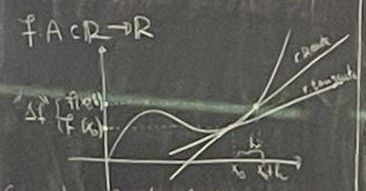
\includegraphics[width = 8cm]{images/derivata.jpeg}
    \caption{Derivata}
    \label{fig:derivata}
\end{figure}

Presa una funzione $y = f (x)$ contenuta in un intervallo $[a,b]$ fissiamo un punto $x_0$ e un incremento destro $h\neq 0$ che mi permette di definire il rapporto incrementale come:
\begin{equation}
    \frac{\Delta y}{\Delta x}=\frac{f(x_0+h)-f(x_0)}{x_0+h-x_0}=\frac{f(x_0+h)-f(x_0)}{h}
\end{equation}

Il rapporto incrementale equivale alla pendenza della retta secante nei punti $(x_0,f(x_0))$ e $(x_0+h,f(x_0+h))$.

Ora voglio calcolare la pendenza della retta tangente. Lo faccio mandando $h$ a zero, ovvero prendendo $\lim_{h\to0}$ del rapporto incrementale e lo chiamo $f'(x_0):=\lim_{h\to0}\frac{h(x_0+h)-f(x_0)}{h}$. Se il limite esiste dico che $f$ è derivabile in $x_0$ e $f'(x_0)$ è la sua derivata.

\begin{osservation}
    Posso anche scrivere i rapporti incrementali come $\frac{f(x)-f(x_0)}{x-x_0}$. Le due definizioni sono infatti equivalenti.
\end{osservation}

Ora, se vogliamo calcolare la derivata in un punto dobbiamo, dobbiamo risolvere il limite della forma indeterminata.

\begin{example}
$f(x)=x^2$ $\hspace{0.5cm}f'(x)=\lim_{x\to x_0}\frac{x^2-x_0}{x-x_0}=\frac{0}{0}$ $\lim_{h\to x_0}\frac{(x_0+h)^2-x_0^2}{h}=\lim_{h\to x_0}\frac{x_0^2+2hx_0+h^2-x_0^2}{h}$ semplificando otteniamo $\lim_{h\to x_0}2x_0+h=\lim_{h\to x_0}2x_0$.
\end{example}
\begin{example}
$f(x)=|x|$ $\hspace{0.5cm}f'(x)=\lim_{x\to 0}\frac{|x|-|0|}{x-0}=\lim_{x\to 0}\frac{|x|}{x}$ non esiste perchè $\lim_{x\to 0^+}\frac{x}{x}=1$ mentre $\lim_{x\to 0^-}\frac{x}{x}=-1$.
\end{example}

\section{Derivabilità implica continuità}
    Se $f$ è derivabile in $x_0$ allora $f$ è continua in $x_0$.
    \begin{dimostration}
        Supponiamo che esista $f'(x_0)=\lim_{x\to x_0}\frac{f(x)-f(x_0)}{x-x_0}$.
        
        Affermo che $f(x)=f(x_0)+f'(x_0)(x-x_0)$ + un termine di errore $e(x)$ con $e(x)\to 0$ per $x\to x_0$ più rapidamente di $x-x_0$. Ovvero $\lim_{x\to x_0}\frac{e(x)}{x-x_0}=0$.
        
        Otteniamo così che $\lim_{x\to x_0}\frac{e(x)}{x-x_0}=\lim_{x\to x_0}\frac{f(x)-f(x_0)}{x-x_0}-f'(x_0)$.
        Notiamo come il rapporto è in realtà la forma della derivata di $f(x)$ quindi otteniamo $\lim_{x\to 0}f'(x_0)-f'(x_0)=0$.
        
        In particolare $\lim_{x\to x_0}e(x)$ moltiplico e divido per $\frac{x-x_0}{x-x_0}$ per ottenere il limite notevole. $\lim_{x\to x_0}e(x)\frac{x-x_0}{x-x_0}$ dove $\frac{e(x)}{x-x_0}$ tende a 0 per il limite notevole mentre $x-x_0$ al numeratore tende a 0 quindi il limite vale 0.
        
        Infine
        \begin{equation*}
            \lim_{x\to x_0}f(x_0)+f'(x_0)(x-x_0)+e(x)=f(x_0)
        \end{equation*}
        Perche i due termini $f'(x_0)(x-x_0)$ e $e(x)$ tendono a 0 come dimostrato prima.
        
        In conclusione ottenendo $\lim_{x\to x_0}f(x)=f(x_0)$ possiamo dire che $f$ è continua in $x_0$. \flushright{$\blacksquare$}
    \end{dimostration}

\section{Derivata di una funzione}
Data $f A\subset \mathbb{R}\to\mathbb{R}$ se $f$ è derivabile in ogni punto di $A$ posso calcolare $f'(x_0)$, $\forall x_0\in A$. Poichè la derivata di $f'(x_0)$ di $f$ in $x_0$ dipende dal punto $x_0$ è essa stessa una funzione che chiamo derivata di $f$.
\begin{notation}
    Si può indicare la derivata anche come:
    \begin{equation*}
        f'(x)=\frac{d}{dx}f(x)=\frac{df}{dx}(x)=\frac{df(x)}{dx}
    \end{equation*}
    
    \begin{example}
        $\frac{d\sin{x}}{dx}=\lim_{h\to0}\frac{\sin{(x+h)}-\sin{x}}{h}=\lim_{h\to0}\frac{\sin{h}\cos{x}+\cos{h}\sin{x}-\sin{x}}{h}=\lim_{h\to0}\frac{\sin{h}\cos{x}}{h}+\frac{(\cos{h-1})\sin{x}}{h}$ applicando i limiti notevoli e moltiplicando e dividento per $h$ otteniamo:
        $\lim_{h\to0}1*\cos{x}+\frac{1(\sin{x})(h)}{2}$
        
        Quindi:
        \begin{equation*}
            \frac{d\sin(x)}{dx}=\cos{x}
        \end{equation*}
    \end{example}
\end{notation}

Possiamo così calcolare le derivate per tutte le principali funzioni:
\begin{table}[ht]
    \centering
    \begin{tabular}{|c|c|}
        \hline\multicolumn{2}{|c|}{\textbf{Fondamentali}}\\\hline\hline
        k &k\\\hline
        x&1\\\hline
        kf(x)&kf'(x)\\\hline
    \end{tabular}
    \caption{Derivate fondamentali}
    \label{tab:deriv_fondam}
\end{table}

\begin{table}[ht]
    \centering
    \begin{tabular}{|c|c||c|c|}
         \hline\multicolumn{2}{|c|}{\textbf{Semplici}} & \multicolumn{2}{|c|}{\textbf{Composte}}\\\hline\hline
         $x^{n}$ & $nx^{n-1}$ & $(f(x))^{n}$ & $n(f(x))^{n-1}f'(x)$\\\hline
         $\sqrt{x}$ & $\frac{1}{2\sqrt{x}}$ & $\sqrt{f(x)}$ & $\frac{1}{2\sqrt{f(x)}}f'(x)$\\\hline
         $\sqrt[n]{x}$ & $\frac{1}{n\sqrt[n]{x^{n-1}}}$ & $\sqrt[n]{f(x)}$ & $\frac{1}{n\sqrt[n]{(f(x))^{n-1}}}f'(x)$\\\hline
         $sinx$ & $cosx$ & $sin(f(x))$ & $cos(f(x))f'(x)$\\\hline
         $cosx$ & $-sinx$ & $cos(f(x))$ & $-f'(x)sin(f(x))$\\\hline
         $e^{x}$ & $e^{x}$ & $e^{f(x)}$ & $f'(x)e^{f(x)}$\\\hline
         $a^{x}$ & $a^{x}\ln{a}$ & $a^{f(x)}$ & $(a^{f(x)}\ln{a})f'(x)$\\\hline
         $\log_{a}{x}$ & $\frac{1}{x}\log_{a}{e}$ & $\log_{a}{f(x)}$ & $\frac{1}{f(x)}\log_{a}{e}f'(x)$\\\hline
         $\ln{x}$ & $\frac{1}{x}$ & $\ln{f(x)}$ & $\frac{f'(x)}{f(x)}$\\\hline
         $tanx$ & $\frac{1}{cos^{2}x}$ & $tan(f(x))$ & $\frac{f'(x)}{cos^{2}(f(x))}$\\\hline
    \end{tabular}
    \caption{Derivate semplici e composte}
    \label{tab:deriv_sem_e_comp}
\end{table}

Abbiamo visto i limiti notevoli per calcolare le derivate di alcune funzioni elementari. Ma come si possono calcolare le derivate di funzioni più complesse?

\subsection{Operazioni con le derivate}
    Se $f$ e $g$ sono derivabili in $x_0$ allora anche $f+g$, $f*g$, $\frac{f}{g}$ sono derivabili in $x_0$. Se ciò è vero possiamo calcolare:
    \begin{align}
        (f+g)'(x_0)=f'(x_0)+g'(x_0)\\
        (fg)'(x_0)=f'(x_0)g(x_0)+f(x_0)g'(x_0)\\
        (\frac{f}{g})'(x_0)=\frac{f'(x_0)g(x_0)-f(x_0)g'(x_0)}{g(x_0)^2}\\
        (f^{-1})'(f(x_0))=\frac{1}{f'(x_0)}
    \end{align}
    \begin{example}
        $\frac{d}{dx}(\cos{x}\ln{x})=-\sin{x}\ln{x}+\frac{\cos{x}}{x}$
        
        $\frac{d}{dx}\tan{x}=\frac{d}{dx}\frac{\sin{x}}{\cos{x}}=\frac{\cos{x}\cos{x}-\sin{x}(-\sin{x})}{\cos^2{x}}=\frac{\cos^2{x}+\sin^2{x}}{\cos^2{x}}=\frac{1}{\cos^2{x}}$
    \end{example}
    \begin{dimostration}[Forma di Leibniz]
        $(fg)'(x_0)=\lim_{x\to x_0}\frac{f(x)g(x)-f(x_0)g(x_0)}{x-x_0}$ sommiamo e sottraiamo $f(x_0)g(x)$ e otteniamo $\lim_{x\to x_0}\frac{f(x)g(x)-f(x_0)g(x)+f(x_0)g(x)-f(x_0)g(x_0)}{x-x_0}=\lim_{x\to x_0}\frac{g(x)(f(x))-f(x_0))}{x-x_0}+\frac{f(x)(g(x)-g(x_0))}{x-x_0}$ notiamo come le due quantità $\frac{f(x))-f(x_0)}{x-x_0}$ e $\frac{g(x)-g(x_0)}{x-x_0}$ equivalgono rispettivamente a $f'(x_0)$ e $g'(x_0)$. Otteniamo così:
        \begin{equation*}
            \lim_{x\to x_0}f'(x_0)g(x)+f(x)g'(x_0)
        \end{equation*}
    \end{dimostration}
\begin{dimostration}[Formula del quoziente]
    Parto da un caso particolare: $f=1$.
    
    $(\frac{1}{g})'=-\frac{1}{g^2}g'$.
    
    $\frac{1}{g}=(h\circ g)$ applico la regola della catena $h'(g(x))=\frac{1}{(g(x))^2}$. Per ottenere la formula del quoziente completa applichiamo Leibniz scrivendo $\frac{f}{g}=f\frac{1}{g}=\frac{f'}{g}+f(-\frac{g'}{g^2})=\frac{f'}{g}-\frac{fg'}{g^2}=\frac{f'g-fg'}{g^2}$
\end{dimostration}


\subsubsection*{Regola della catena}
C'è inoltre un'altra formula introdotta con la regola della catena.
Siano $f$ derivabile in $x_0$ e $g$ derivabile in $y_0=f(x_0)$, allora $g\circ f$ è derivabile in $x_0$ e vale:
\begin{equation}
    (g\circ f)'(x_0)=g'(f(x_0))(f'(x_0))
\end{equation}

\begin{example}
    $\frac{d}{dx}(\cos{(x^2)})$
    $f(x)=x^2\hspace{0,5cm}g(y)=\cos{(y)}\hspace{0,5cm}f'(x)=2x\hspace{0,5cm}g'(x)=-\sin{(y)}$
    
    $\frac{d}{dx}(\cos{(x^2)})=-\sin{x^2}2x$
\end{example}

\section{Massimi e minimi con derivate}
\subsection{Teorema di Fermat}
\begin{definition}[Massimi e minimi relativi]
    Data $fA\subset\mathbb{R}\to\mathbb{R}$, $x_0$ si dice punto di $\max, \min$ relativo se $\exists\delta>0\text{ t.c. }f(x_0)\geq f(x)$, $\forall x\in A\cup\{x_0-\delta,x_0+\delta\}$.
\end{definition}

\begin{definition}[Massimi e minimi assoluti]
    $x_0$ si dice punto di $\max, \min$ assoluto se $\exists\delta>0\text{ t.c. }f(x_0)\geq f(x)$, $\forall x\in A$.
\end{definition}

\begin{center}
    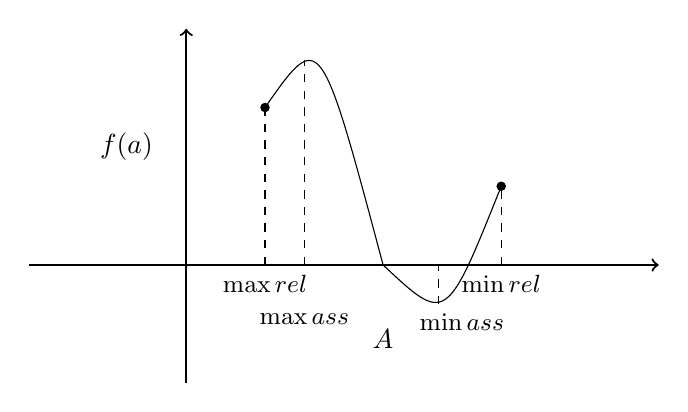
\begin{tikzpicture}
        % Assi
        \draw [->,thick] (1,1) -- (9,1);
        \draw [->,thick] (3,-0.5) -- (3,4);
        
        \draw [dashed] (4,1) -- (4,3);
        \draw [dashed] (7,1) -- (7,2);
        
        \draw [dashed] (4.5,1) -- (4.5,3.6);
        \draw [dashed] (6.2,0.5) -- (6.2,1);
        
        \draw (4, 3) .. controls (4.7,4) .. (5.5, 1);
        \draw (5.5, 1) .. controls (6.3,0.25) .. (7,2);
        % Numeri
        \draw (4.5,0.5) -- (4.5,0.5) node [below] {\small{$\max{ass}$}};
        \draw (6.5,0.5) -- (6.5,0.5) node [below] {\small{$\min{ass}$}};
        \draw (4,1) -- (4,1) node [below] {\small{$\max{rel}$}};
        \draw (7,1) -- (7,1) node [below] {\small{$\min{rel}$}};
        \draw (5.5,0.3) -- (5.5,0.3) node [below] {\normalsize{$A$}};
        \draw (2.7,2.5) -- (2.7,2.5) node [left] {\normalsize{$f(a)$}};
        % Punti
        \filldraw[black] (4,3) circle (1.5pt);
        \filldraw[black] (7,2) circle (1.5pt);
    \end{tikzpicture}
\end{center}

All'interno del dominio di A, quando si incontra un punto di massimo o di minimo, la tangente è parallela all'asse delle x, quindi la derivata è uguale a 0.

\begin{thm}
    Sia $f[a,b]\to\mathbb{R}$ e sia $x_0\in(a,b)$, punto di $\max, \min$ relativo. Sia anche $f$ derivabile in $x_0$ allora $f'(x_0)=0$.
    \begin{dimostration}
        Poichè $f$ è derivabile in $x_0$, $\exists\lim_{x\to x_0}\frac{f(x)-f(x_0)}{x-x_0}$.
        
        Sia $x_0$ punto di massimo relativo, allora $f(x)\leq f(x_0)$ per $x$ vicino a $x_0$.
        Quindi se esiste il limite $\lim_{x\to x_0}\frac{f(x)-f(x_0)}{x-x_0}$ allora esiste per $(x,x+\delta)$:
        \begin{equation*}
            f'(x_0)=\lim_{x\to x_0^+}\frac{f(x)-f(x_0)}{x-x_0}\leq0
        \end{equation*}
        Allo stesso modo esiste per $(x,x+\delta)$:
        \begin{equation*}
            f'(x_0)=\lim_{x\to x_0^-}\frac{f(x)-f(x_0)}{x-x_0}\geq0
        \end{equation*}
        
        Quindi $f'(x_0)=0$.
    \end{dimostration}
\end{thm}

\begin{definition}[Punto critico]
    Un punto $x_0$ t.c. $f'(x_0)=0$ si dice punto critico.
    \begin{osservation}
        Non tutti i punti critici sono di massimo e di minimo.
        
        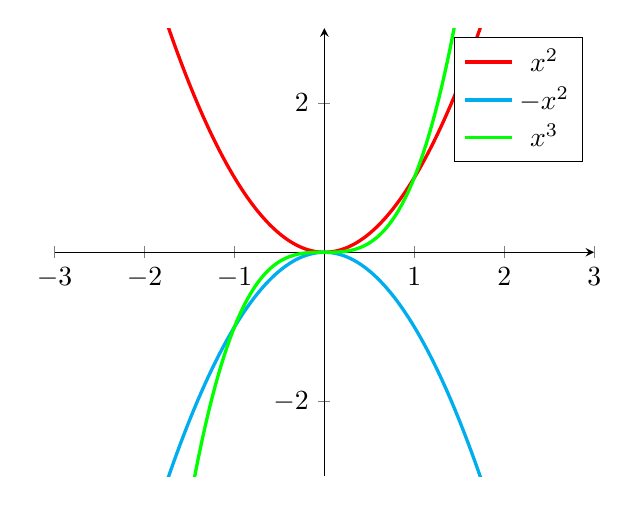
\begin{tikzpicture}
            \begin{axis}[xmin=-3,xmax=3,ymin=-3,ymax=3,axis x line=middle, axis y line=middle]
            \addplot [very thick,domain=-5:5,samples=500,color=red,]{x^2};\addlegendentry{$x^2$}
            \addplot [very thick,domain=-5:5,samples=500,color=cyan,]{-x^2};\addlegendentry{$-x^2$}
            \addplot [very thick,domain=-5:5,samples=500,color=green,]{x^3};\addlegendentry{$x^3$}
            \end{axis}
        \end{tikzpicture}
        
        Notiamo come per $x=0$ punto critico le funzioni $x^2$ e $-x^2$ hanno rispettivamente $\max, \min$, mantre la funzione $x^3$ non ha nè $\max$ nè $\min$.
    \end{osservation}
\end{definition}

\section{Teorema di Rolle}
Sia $f\in C^\circ([a,b])$ derivabile in $(a,b)$ t.c. $f(a)=f(b)$ allora:
\begin{equation}
    \exists\xi\in(a,b)\text{ t.c. }f'(\xi)=0
\end{equation}

\begin{figure}[ht]
    \centering
    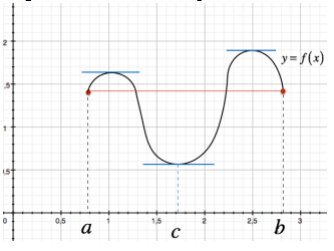
\includegraphics[width = 6cm]{images/rolle.png}
    \caption{Teorema di Rolle}
\end{figure}

\begin{dimostration}
    Se troviamo un punto di $\min, \max$ interni possiamo applicare il teorema di Fermat:
    \begin{itemize}
        \item[Caso 1)] $\max_[a,b] f>f(a)$ allora $x_M\in(a,b)$
        \begin{equation*}
            f'(x_M)=0 \text{ scelgo } \xi=x_M
        \end{equation*}
        \item[Caso 2)] $\max_[a,b] f=f(a)$ però $\min_[a,b] f<f(a)$ allora $x_M\in(a,b)$
        \begin{equation*}
            f'(x_m)=0 \text{ scelgo } \xi=x_m
        \end{equation*}
        \item[Caso 3)] $\max f=f(a)=\min f$ in questo caso
        \begin{equation*}
            f'(x)=0 \forall x\in(a,b) \text{ scelgo } \xi\in(a,b) \text{ qualsiasi.}
        \end{equation*}
    \end{itemize}\flushright{$\blacksquare$}
\end{dimostration}

\section{Teorema di Lagrange}
Sia $f\in C^\circ([a,b])$ derivabile in $(a,b)$ allora $\exists\xi\in(a,b)$ t.c.:
\begin{equation}
    f'(\xi)=\frac{f(b)-f(a)}{b-a}
\end{equation}
Rappresenta la pendenza della retta secante.

\begin{figure}[ht]
    \centering
    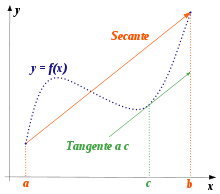
\includegraphics[width = 6cm]{images/lagrange.png}
    \caption{Teorema di Lagrange}
\end{figure}

\begin{dimostration}
    Introduciamo la funzione $h(x)=f(x)-\frac{f(b)-f(a)}{b-a}(x-a)$ otteniamo che $h(x)\in C^\circ([a,b])$ perchè differenza di due funzioni continue ed è anche derivabile per lo stesso motivo.
    
    $h(a)=f(a)\hspace{0,5cm}h(b)=f(b)-\frac{f(b)-f(a)}{b-a}(b-a)=f(a)$ quindi $h(a)=h(b)$. Applico il teorema di Rolle perchè $h$ soddisfa tutte le condizioni: $h'(\xi)=0$.
    
    Infine otteniamo $h'(\xi)=f'(\xi)-\frac{f(b)-f(a)}{b-a}*1$
    
    $f'(\xi)=\frac{f(b)-f(a)}{b-a}$\flushright{$\blacksquare$}
\end{dimostration}

\begin{proposition}
    Sia $f:I\in\mathbb{R}\to\mathbb{R}$ t.c. $f'(x)=0\forall x\in I$. Allora $f$ è costante.
    \begin{dimostration}
        Siano $a,b\in I$ con $a<b$, applico il teorema di Lagrange, $f'(\xi)=\frac{f(b)-f(a)}{b-a}$, ma $f'(\xi)=0$ per ipotesi quindi anche $\frac{f(b)-f(a)}{b-a}=0$. Da ciò ne ricavo che $f(b)-f(a)=0$ e $f(b)=f(a)$.
    \end{dimostration}
\end{proposition}

\begin{proposition}
    Sia $f:I\in\mathbb{R}\to\mathbb{R}$ derivabile con $f'(x)\geq0\forall x\in I$. Allora f è monotona crescente.
    
    \begin{dimostration}
    Siano $a,b\in I$ con $a<b$, applico il teorema di Lagrange, $f'(\xi)=\frac{f(b)-f(a)}{b-a}$, ma $f'(\xi)\geq0$ per ipotesi quindi anche $\frac{f(b)-f(a)}{b-a}\geq0$. Da ciò ne ricavo che $f(b)-f(a)\geq0$ e $f(b)\geq f(a)$.
    
    Questo vale per ogni coppia $(a,b)\in I$ con $a<b$ quindi la funzione è monotona crescente.
    
    Lo stesso vale per $f'(x)\leq0\forall x\in I$ f è decrescente.
    \end{dimostration}
\end{proposition}

\subsection{Intervalli di monotonia}
Gli intervalli di monotonia sono intervalli in cui $f'\geq0$ o $f'\leq0$ quindi f è crescente o decrescente.
\begin{example}
    $f(x)=x^2-5x+6$ vogliamo trovare gli intevalli di monotonia.
    
    Dominio $=\mathbb{R}$ $f'(x)=2x-5\leq0$ se $2x\leq5$ quindi per $x\leq\frac{5}{2}$ abbiamo ottenuto che la funzione decresce da $-\infty$ a $\frac{5}{2}$, mentre cresce da $\frac{5}{2}$ a $+\infty$.
\end{example}

\begin{proposition}
    $f,g\in C^\circ[a,b]$ derivabile in $(a,b)$ supponiamo che $f(a)\geq g(a)$ e $f'(x)\geq g'(x)\forall x\in(a,b)$, allora $f(x)\geq g(x)\forall x\in[a,b]$.
    \begin{dimostration}
        Poniamo $h(x)=f(x)-g(x)$ con $h(x)\in C^\circ[a,b]$ derivabile in $(a,b)$
        
        $h'(x)=f'(x)-g'(x)\geq0$ quindi h è crescente in $(a,b)$. Ma $h(a)=f(a)-g(a)\geq0$ con $h(x)\geq0$ otteniamo $f(x)\geq g(x)$.
    \end{dimostration}
\end{proposition}

\section{Teorema di de l'Hopital}
Il teorema di De Hospital viene utilizzato per i limti che come risultato presentano una forma indeterminata $\frac{0}{0}$ o $\frac{\infty}{\infty}$.

$f,g:[a,b]\to\mathbb{R}$ derivabili in $(a,b)$ t.c.
\begin{enumerate}
    \item $f(a)=g(a)=0$
    \item $g'(x)\neq0$, $\forall x\in (a,b)$
    \item $\exists\lim_{x\to a}\frac{f'(x)}{g'(x)}=l$
\end{enumerate}

Allora:
\begin{equation}
    \lim_{x\to a}\frac{f(x)}{g(x)}=l
\end{equation}

\begin{example}
    $\lim_{x\to0}\frac{\sin (2x)}{x}=2$
    
    $\lim_{x\to0}\frac{f'(x)}{g'(x)}=\lim_{x\to0}\frac{2\cos(2x)}{1}=2$
\end{example}